\documentclass[10pt,landscape,a4paper]{article}
\usepackage[utf8]{inputenc}
\usepackage[T1]{fontenc}
\usepackage{tikz}
\usetikzlibrary {3d, intersections}
\usepackage{kpfonts}
\usepackage{multicol}
\usepackage{wrapfig}
\usepackage[top=1mm,bottom=1mm,left=1mm,right=1mm]{geometry}
\usepackage[framemethod=tikz]{mdframed}
\usepackage{pdfpages}
\usepackage{amsmath}
\usepackage{amsfonts}
\usepackage{pgfplots}
\pgfplotsset{compat=1.15}
\usepackage{caption}
\usepackage{graphicx}

\newenvironment{Figure}
  {\par\medskip\noindent\minipage{\linewidth}}
  {\endminipage\par\medskip}

\newcommand{\header}{
\begin{mdframed}[style=header]
\footnotesize
\sffamily
MA1521 Cheatsheet\\
Donk,~page~\thepage~of~2
\end{mdframed}
}

\definecolor{myblue}{cmyk}{1,.72,0,.38}

\def\multi@column@out{%
   \ifnum\outputpenalty <-\@M
   \speci@ls \else
   \ifvoid\colbreak@box\else
     \mult@info\@ne{Re-adding forced
               break(s) for splitting}%
     \setbox\@cclv\vbox{%
        \unvbox\colbreak@box
        \penalty-\@Mv\unvbox\@cclv}%
   \fi
   \splittopskip\topskip
   \splitmaxdepth\maxdepth
   \dimen@\@colroom
   \divide\skip\footins\col@number
   \ifvoid\footins \else
      \leave@mult@footins
   \fi
   \let\ifshr@kingsaved\ifshr@king
   \ifvbox \@kludgeins
     \advance \dimen@ -\ht\@kludgeins
     \ifdim \wd\@kludgeins>\z@
        \shr@nkingtrue
     \fi
   \fi
   \process@cols\mult@gfirstbox{%
%%%%% START CHANGE
\ifnum\count@=\numexpr\mult@rightbox+2\relax
          \setbox\count@\vsplit\@cclv to \dimexpr \dimen@-1cm\relax
\setbox\count@\vbox to \dimen@{\vbox to 1cm{\header}\unvbox\count@\vss}%
\else
      \setbox\count@\vsplit\@cclv to \dimen@
\fi
%%%%% END CHANGE
            \set@keptmarks
            \setbox\count@
                 \vbox to\dimen@
                  {\unvbox\count@
                   \remove@discardable@items
                   \ifshr@nking\vfill\fi}%
           }%
   \setbox\mult@rightbox
       \vsplit\@cclv to\dimen@
   \set@keptmarks
   \setbox\mult@rightbox\vbox to\dimen@
          {\unvbox\mult@rightbox
           \remove@discardable@items
           \ifshr@nking\vfill\fi}%
   \let\ifshr@king\ifshr@kingsaved
   \ifvoid\@cclv \else
       \unvbox\@cclv
       \ifnum\outputpenalty=\@M
       \else
          \penalty\outputpenalty
       \fi
       \ifvoid\footins\else
         \PackageWarning{multicol}%
          {I moved some lines to
           the next page.\MessageBreak
           Footnotes on page
           \thepage\space might be wrong}%
       \fi
       \ifnum \c@tracingmulticols>\thr@@
                    \hrule\allowbreak \fi
   \fi
   \ifx\@empty\kept@firstmark
      \let\firstmark\kept@topmark
      \let\botmark\kept@topmark
   \else
      \let\firstmark\kept@firstmark
      \let\botmark\kept@botmark
   \fi
   \let\topmark\kept@topmark
   \mult@info\tw@
        {Use kept top mark:\MessageBreak
          \meaning\kept@topmark
         \MessageBreak
         Use kept first mark:\MessageBreak
          \meaning\kept@firstmark
        \MessageBreak
         Use kept bot mark:\MessageBreak
          \meaning\kept@botmark
        \MessageBreak
         Produce first mark:\MessageBreak
          \meaning\firstmark
        \MessageBreak
        Produce bot mark:\MessageBreak
          \meaning\botmark
         \@gobbletwo}%
   \setbox\@cclv\vbox{\unvbox\partial@page
                      \page@sofar}%
   \@makecol\@outputpage
     \global\let\kept@topmark\botmark
     \global\let\kept@firstmark\@empty
     \global\let\kept@botmark\@empty
     \mult@info\tw@
        {(Re)Init top mark:\MessageBreak
         \meaning\kept@topmark
         \@gobbletwo}%
   \global\@colroom\@colht
   \global \@mparbottom \z@
   \process@deferreds
   \@whilesw\if@fcolmade\fi{\@outputpage
      \global\@colroom\@colht
      \process@deferreds}%
   \mult@info\@ne
     {Colroom:\MessageBreak
      \the\@colht\space
              after float space removed
              = \the\@colroom \@gobble}%
    \set@mult@vsize \global
  \fi}

\makeatother
\setlength{\parindent}{0pt}

\makeatletter
\renewcommand{\section}{\@startsection{section}{1}{0mm}%
                                {.2ex}%
                                {.2ex}%x
                                {\color{myblue}\sffamily\small\bfseries}}
\renewcommand{\subsection}{\@startsection{subsection}{1}{0mm}%
                                {.2ex}%
                                {.2ex}%x
                                {\sffamily\bfseries}}


\begin{document}
\small
\begin{multicols*}{4}

\section{Limits and Continuity}
$\lim_{x\to a} f(x)$ exists$\Leftrightarrow\lim_{x\to a^+}f(x)=\lim_{x\to a^-}f(x)$\\
\textbf{Continuity at x = c}$\Leftrightarrow\lim_{x\to a}f(x)=L=f(c)$\\
\textbf{Continuity at endpoints} only one-sided limit.\\
\textbf{Continuity at an interval}$\Leftrightarrow \forall c\in I(f$ is continuous at $c)$\\
\textbf{Squeeze Theorem}\\
$Let\ I=(a,c)\cup(c,b).\ \forall x\in I(f(x)\le g(x)\le h(x))$\\
$\lim_{x\to c}f(x)=\lim_{x\to c}h(x)=L\Rightarrow\lim_{x\to c}g(x)=L$\\
\textbf{Special Limit}\\$\lim_{x\to c}g(x)=0\Rightarrow\lim_{x\to c}\frac{\sin(g(x))}{g(x)}=\lim_{x\to c}\frac{\tan(g(x))}{g(x)}=1$\\
\textbf{Indeterminate Limit}\\$\lim_{x\to c}\frac{f(x)}{g(x)}$ $\Rightarrow\lim_{x\to c}\frac{f(x)}{g(x)}=\lim_{x\to c}\frac{f'(x)}{g'(x)}$
\section{Theorems}
\textbf{Intermediate Value Theorem}\\ $f$ is continuous on $[a,b]$, $k\in[f(a),f(b)]\Rightarrow\exists c\in [a,b](f(c)=k)$\\
\textbf{Rolle's Theorem}\\$f$ is differentiable on $(a,b)$, $f(a)=f(b)\Rightarrow\exists c\in(a,b)(f'(c)=0)$\\
\textbf{Mean Value Theorem}\\$f$ is differentiable on $(a,b)$, $\exists c\in(a,b)(f'(c)=\frac{f(b)-f(a)}{b-a})$
\section{Derivative}
\textbf{Limit Definition}\\$f'(x_0)=\lim_{h\to 0}\frac{f(x_0+h)-f(x_0)}{h}$\\
\textbf{Differentiability on an Interval}$\Leftrightarrow$ Continuous on the interval\\
\textbf{Quotient Rule}\\$\frac{d}{dx}(\frac{u}{v})=\frac{\frac{du}{dx}\cdot v-\frac{dv}{dx}\cdot u}{v^2}$\\
\textbf{Inverse Derivative}\\$(f^{-1})'(a)=\frac{1}{f'(f^{-1}(a))}$\\
\textbf{Derivative of Parametric}\\$\frac{dy}{dx}=\frac{g'(t)}{f'(t)}$\\
$\frac{d^2y}{d^2x}=\frac{f'(t)\cdot g''(t)-f''(t)\cdot g'(t)}{(f'(t))^3}$\\
\textbf{Critical Point}\\Not end point, $f'(c)=0\vee f'(c)$ does not exist.\\
\textbf{Absolute Extrema by First Derivative}\\
$\forall x<c(f'(x)>0)\wedge\forall x>c(f'(x)<0)\Rightarrow f$ has an absolute maximum at $c$\\
$\forall x<c(f'(x)<0)\wedge\forall x>c(f'(x)>0)\Rightarrow f$ has an absolute minimum at $c$\\
\textbf{Local Extrema by First Derivative}\\
$f$ is differentiable on $(a,c)\cup(c,b)\wedge$ continuous at $c$\\
$f'$ changes from $+$ to $-$ at $x=c\Rightarrow$ max\\
$f'$ changes from $-$ to $+$ at $x=c\Rightarrow$ min\\
\textbf{Second Derivative Test}\\
$f'(c)=0\wedge f''(c)<0\Rightarrow$local max at $c$\\
$f'(c)=0\wedge f''(c)>0\Rightarrow$local min at $c$\\
\section{Integration}
\textbf{Partial Fractions}
Simplify $\frac{P(x)}{Q(x)}$
\begin{center}
   \begin{tabular}{|c|c|}
      \hline
      \multicolumn{2}{|c|}{Factors of $Q(x)$}\\
      \hline
      $ax+b$ & $\frac{A}{ax+b}$\\
      $(ax+b)^2$ & $\frac{A}{ax+b}+\frac{B}{(ax+b)^2}$\\
      $ax^2+bx+c$ & $\frac{Ax+B}{ax^2+bx+c}$\\
      \hline
   \end{tabular}
\end{center}
\textbf{Trigo Substitution}
\begin{center}
   \begin{tabular}{|c|c|}
      \hline
      Expression & Substitution\\
      \hline
      $\sqrt{a^2-(x+b)^2}$ & $x+b=a\sin\theta$\\
      $\sqrt{(x+b)^2+a^2}$ & $x+b=a\tan\theta$\\
      $\sqrt{(x+b)^2-a^2}$ & $x+b=a\sec\theta$\\
      \hline
   \end{tabular}
\end{center}
Domains: $-\frac{\pi}{2}\le\theta\le\frac{\pi}{2}$,$-\frac{\pi}{2}<\theta<\frac{\pi}{2}$,$0<\theta<\frac{\pi}{2}$ OR $\pi\le\theta<\frac{3\pi}{2}$\\
\textbf{Integration by Parts}\\
$\int f'(x)g(x)dx=f(x)g(x)-\int f(x)g'(x)dx$\\
(diff) Log, Inverse, Alge, Trig, Expo (int)\\
\textbf{Riemann Sum}\\
$\int_{a}^{b}f(x)dx=\lim_{n\to\infty}{\sum_{k=1}^{n}(\frac{b-a}{n})f(a+k(\frac{b-a}{n}))}$\\
\textbf{Fundamental Theorem of Calculus}\\
$\int_{a}^{b}f(x)dx=F(b)-F(a)$\\
\textbf{Second Fund. Theorem of Calc}\\
$F(x)=\int_{a}^{x}f(t)dt,a\le x\le b,F(a)=0$\\
$\frac{d}{dx}\int_{a}^{x}f(t)dt=f(x)$\\
\textbf{Improper Integrals}\\
$\int_{-\infty}^{\infty}f(x)dx=\lim_{a\to -\infty}\int_{a}^{c}f(x)dx+\lim_{b\to\infty}\int_{c}^{b}f(x)dx$\\
$\int_{a}^{b}f(x)dx=\lim_{c\to d^-}\int_{a}^{c}f(x)dx+\lim_{c\to d^+}\int_{c}^{b}f(x)dx$
\section{Integration Applications}
\textbf{Area between curves}\\
$\int_{a}^{b}\left|f(x)-g(x)\right|dx$, $\int_{a}^{b}\left|f(y)-g(y)\right|dy$\\
\textbf{Volume of Solid by Disk}\\
$\pi\int_{a}^{b}f(x)^2dx-\pi\int_{a}^{b}g(x)^2dx$\\
$\pi\int_{a}^{b}f(y)^2dy-\pi\int_{a}^{b}g(y)^2dy$\\
\textbf{Volume of Solid by Cyindrical Shell}\\
$2\pi\int_{a}^{b}x\left|f(x)-g(x)\right|dx$\\
$2\pi\int_{a}^{b}y\left|f(y)-g(y)\right|dy$\\
\textbf{Length of curve y=f(x)}\\
$\int_{a}^{b}\sqrt{1+f'(x)^2}dx$,
$\int_{p}^{q}\sqrt{1+f'(y)^2}dy$
\section{Equations}
\textbf{Ellipse} $\frac{(x-x_0)^2}{a^2}+\frac{(y-y_0)^2}{b^2}=1$\\
$x=a\cos(t)+x_0, y=b\sin(t)+y_0$\\
\textbf{Circle} $(x-x_0)^2+(y-y_0)^2=r^2$\\
$x=r\cos(t)+x_0, y=r\sin(t)+y_0$\\
\textbf{Horizontal Hyperbola}\\
$\frac{(x-x_0)^2}{a^2}-\frac{(y-y_0)^2}{b^2}=1$\\
$x=a\sec(t)+x_0,y=b\tan(t)+y_0$\\
\textbf{Vertical Hyperbola}\\
$\frac{(y-y_0)^2}{b^2}-\frac{(x-x_0)^2}{a^2}=1$\\
$x=a\tan(t)+x_0,y=b\sec(t)+y_0$
\section{Series}
\textbf{Convergence of series}
$\lim_{n\to\infty}a_n=L$\\
\textbf{Absolute Convergence}
$\sum_{n=1}^{\infty}\left|a_n\right|$ is convergent.
\textbf{Geometric Series} Convergent for $\left|r\right|<1$
\[\sum_{i=1}^{n}ar^{i-1}=\begin{cases}
   \frac{a(1-r^n)}{1-r} & if r\neq1\\
   an & if r = 1
\end{cases}\]
\textbf{p-series}
$\sum_{n=1}^{\infty}\frac{1}{n^p}$ convergent $\Leftrightarrow p>1$\\
\section{Tests for Convergence}
\textbf{n-th Term Test}\\
$\lim_{n\to\infty}a_n\neq0\vee\lim_{n\to\infty}a_n DNE\Rightarrow\sum_{n=1}^{\infty}a_n$ is divergent.\\
\textbf{Convergence by Partial Sum}\\
$\forall n\in\mathbb{N}\ \exists k\in\mathbb{R}(S_n<k)\Leftrightarrow\sum_{n=1}^{\infty}a_n$ of non-negative terms converge\\
\textbf{Integral Test}\\
$\forall n\in\mathbb{N}(a_n=f(n)), \forall x\ge1(f(x)$ is continuous, positive, decreasing$)$\\
$\sum_{n=1}^{\infty}a_n$ is convergent$\Leftrightarrow\int_{1}^{\infty}f(x)$ is convergent\\
\textbf{Comparison Test}\\
$\forall n\in\mathbb{N}(0\le a_n\le b_n)$\\
$\sum_{n=1}^{\infty}a_n$ is divergent$\Rightarrow\sum_{n=1}^{\infty}b_n$ is divergent.\\
$\sum_{n=1}^{\infty}b_n$ is convergent$\Rightarrow\sum_{n=1}^{\infty}a_n$ is convergent.\\
\textbf{Ratio/Root Test}\\
$\lim_{n\to\infty}\left|\frac{a_{n+1}}{a_n}\right|=L$ OR $\lim_{n\to\infty}\sqrt[n]{\left|{a_n}\right|}=L$,\\
$0\le L<1\Rightarrow\sum_{n=1}^{\infty}a_n$ is absolutely convergent.\\
$L>1\Rightarrow\sum_{n=1}^{\infty}a_n$ is divergent.\\
$L=1$ is inconclusive.\\
\textbf{Alternating Series Test}\\
$\forall n\in\mathbb{N}(b_n>0\wedge b_n\ge b_{n+1})\wedge \lim_{n\to\infty}b_n=0\Rightarrow$\\
Alternating series\\
$\sum_{n=1}^{\infty}(-1)^{n-1}b_n=b_1-b_2+b_3-b_4+...$ and \\
$\sum_{n=1}^{\infty}(-1)^nb_n=-b_1+b_2-b_3+b_4-...$ are convergent.
\section{Power Series}
\textbf{Deriving Radius of Convergence}:\\Using Ratio or Root Test!\\
\textbf{Radius of Convergence}\\
$\lim_{n\to\infty}\left|\frac{c_{n+1}}{c_n}\right|=\frac{1}{R}$ OR $\lim_{n\to\infty}\sqrt[n]{\left|c_n\right|}=\frac{1}{R}$\\
For $\sum_{n=0}^{\infty}c_n(x-a)^n$,\\$\left|x-a\right|<R$: Absolute Convergence\\
$\left|x-a\right|=R$: Check with Convergence Tests\\
\textbf{Power Series Representation}\\
$\frac{1}{1+x}=\sum_{n=0}^{\infty}(-1)^nx^n$\\
$f(x)=\sum_{n=0}^{\infty}c_n(x-a)^n$\\
$f'(x)=\sum_{n-1}^{\infty}nc_n(x-a)^{n-1}$\\
$\int f(x)=\sum_{n=0}^{\infty}\frac{c_n(x-a)^{n+1}}{n+1}+C$\\
\textbf{Taylor Series} of $f$ at $x=a$
\[f(x)=\sum_{n=0}^{\infty}\frac{f^{(n)}(a)}{n!}(x-a)^n,\ \left|x-a\right|<R\]
\textbf{Maclaurin Series} of $f$ = Taylor Series of $f$ at $a=0$:
\[f(x)=\sum_{n=0}^{\infty}{\frac{f^{(n)}(0)}{n!}(x-a)^n},\ \left|x-a\right|<R\]
\textbf{Common Maclaurin Series}
\begin{itemize}
   \item $\frac{1}{1-x}=1+x+x^2+x^3+...=\sum_{n=0}^{\infty}x^n$
   \item $e^x=1+\frac{x}{1!}+\frac{x^2}{2!}+\frac{x^3}{3!}+...=\sum_{n=0}^{\infty}\frac{x^n}{n!}$
   \item $\sin x=x-\frac{x^3}{3!}+\frac{x^5}{5!}-\frac{x^7}{7!}+...=\sum_{n=0}^{\infty}\frac{(-1)^nx^{2n+1}}{(2n+1)!}$
   \item $\cos x=1-\frac{x^2}{2!}+\frac{x^4}{4!}-\frac{x^6}{6!}+...=\sum_{n=0}^{\infty}\frac{(-1)^nx^{2n}}{(2n)!}$
   \item $\ln(1+x)=x-\frac{x^2}{2}+\frac{x^3}{3}-\frac{x^4}{4}+...=\sum_{n=0}^{\infty}\frac{(-1)^nx^{n+1}}{n+1}$
\end{itemize}
\section{3D Coordinate System}
\textbf{Distance betwen points}\\
$D=\sqrt{(x_1-x_2)^2+(y_1-y_2)^2+(z_1-z_2)^2}$\\
\textbf{Length of Vector}\\
$\|u\|=\sqrt{u_1^2+u_2^2+u_3^2}$\\
\textbf{Dot Product}\\
$\overrightarrow{a}\cdot\overrightarrow{b}=\|\overrightarrow{a}\|\cdot\|\overrightarrow{b}\|\cdot\cos\theta$\\
$\overrightarrow{a}\cdot\overrightarrow{a}=\|\overrightarrow{a}\|^2$\\
\textbf{Cross Product}\\
Area of a parallelogram with sides $\overrightarrow{a}$ and $\overrightarrow{b}$:\\
$\|\overrightarrow{a}\times\overrightarrow{b}\|=\|\overrightarrow{a}\|\ \|\overrightarrow{b}\|\sin\theta$\\
Distance from Point Q to Line PR:\\
$\frac{\|\overrightarrow{PQ}\times\overrightarrow{PR}\|}{\|\overrightarrow{PR}\|}$\\
\textbf{Angle between Vectors}\\
$\cos\theta=\frac{\overrightarrow{a}\cdot\overrightarrow{b}}{\|\overrightarrow{a }\|\ \|\overrightarrow{b }\|}$\\
$\sin\theta=\frac{\|\overrightarrow{a }\times\overrightarrow{b }\|}{\|\overrightarrow{a }\|\ \|\overrightarrow{b }\|}$\\
\textbf{Projection} of $\overrightarrow{b}$ on $\overrightarrow{a}$\\
Vector Projection $proj_{\overrightarrow{a}}\overrightarrow{b}=\frac{\overrightarrow{a}\cdot\overrightarrow{b}}{\overrightarrow{a}\overrightarrow{a}}\overrightarrow{a}$\\
Scalar Projection $comp_{\overrightarrow{a}}\overrightarrow{b}=\frac{\overrightarrow{a}\cdot\overrightarrow{b}}{\|\overrightarrow{a}\|}$\\
\textbf{Distance between Point and Plane}\\
Plane Equation: $d=ax+by+cz$, Point: $(x_0, y_0, z_0)$\\
$Distance = \frac{|ax_0+by_0+cz_0-d|}{\sqrt{a^2+b^2+c^2}}$\\
\textbf{Cylinder}\\
A surface where $\exists$ Plane P such that all the planes parallel to P intersect the surface in the same curve.
\section{Calculus but 3D :D}
\textbf{Vector-Valued Function}
$f: \mathbb{R}\to\mathbb{V}_n$\\
\textbf{Derivative of Vector-valued Function}\\
$r'(t)=\langle f'(t),g'(t),h'(t)\rangle$\\
\textbf{Arc Length of Curve}\\
$\int_{a }^{b }\sqrt{f'(t)^2+g'(t)^2+h'(t)^2}dt=\int_{a }^{b }\|r'(t)\|dt$\\
\textbf{Tangent line to Curve}\\
$r'(a)$ is the tangent vector to the curve at $a$.\\
Form a line with the origin point at $t=a$ and the tangent vector.\\
\textbf{Differentiability of f(x,y)}\\
Tangent Plane at $x=a, y=b$ is a good approximation to $f$ at points close to $(a,b)$\\
\textbf{Chain Rule but 3D}\\
$z=f(g(t),h(t))\Rightarrow\frac{dz}{dt}=\frac{\partial f }{\partial x}\cdot\frac{dx}{dt}+\frac{\partial f}{\partial y}\cdot\frac{dy}{dt}$\\
$z=f(g(s,t),h(s,t))\Rightarrow\frac{\partial z}{\partial x}=\frac{\partial f }{\partial x}\cdot\frac{\partial x}{\partial s }+\frac{\partial f }{\partial y}\cdot\frac{\partial y}{\partial s}$\\
$z=f(g(s,t),h(s,t))\Rightarrow\frac{\partial z}{\partial x}=\frac{\partial f }{\partial x}\cdot\frac{\partial x}{\partial t}+\frac{\partial f }{\partial y}\cdot\frac{\partial y}{\partial t}$\\
\textbf{Increment/Differential of z}\\
$\triangle z=f(x+\triangle x, y+\triangle y)-f(x,y)$\\
$dz=f_x(x,y)dx+f_y(x,y)dy$\\
\textbf{Gradient of f(x,y)}\\
$\nabla f=\langle f_x,f_y\rangle$ is normal to the level curve $f(x,y)=k$\\
$\nabla f=\langle f_x,f_y,f_z\rangle$ is normal to any curve C on surface S $f(x,y,z)=k$\\
\textbf{Tangent Plane to Surface} $z=f(x,y)$\\
$z=f(a,b)+f_x(a,b)(x-a)+f_y(a,b)(y-b)$\\
\textbf{Tangent Plane to Level Surface}\\
$\nabla f(x_0,y_0,z_0)\cdot\langle x-x_0,y-y_0,z-z_0\rangle=0$\\
$f_x(x_0,y_0,z_0)(x-x_0)+f_y(x_0,y_0,z_0)(y-y_0)+f_z(x_0,y_0,z_0)(z-z_0)=0$\\
\textbf{Direction Derivative of f(x,y)}\\
At $(x_0,y_0)$, in the direction of unit vector $\langle a,b\rangle$:\\
$D_uf(x_0,y_0)=\lim_{h\to0}\frac{f(x_0+ha,y_0+hb)-f(x_0,y_0)}{h}$\\
$D_uf(x,y)=\nabla f\cdot\langle a,b\rangle$\\
\textbf{Maximum Rate of Change of f at point P}\\
$\nabla f$ is maximum ($\|\nabla f(P)\|$) in direction $\nabla f(P)$\\
$\nabla f$ is minimum ($-\|\nabla f(P)\|$) in direction $-\nabla f(P)$\\
\textbf{Critical Points of f(x,y)}\\
$f_x(a,b)=0=f_y(a,b)$ OR $f_x$ or $f_y$ does not exist at $(a,b)$\\
\textbf{Local Maxima, Minima, Saddle Points}\\
$\forall(x,y)$ in a disk with center $(a,b),\ f(x,y)\le f(a,b)\Rightarrow(a,b)$ is a local maximum point, $f(a,b)$ is a local maximum value\\
$\forall(x,y)$ in a disk with center $(a,b),\ f(x,y)\ge f(a,b)\Rightarrow(a,b)$ is a local minimum point, $f(a,b)$ is a local minimum value\\
Critical point, $\forall$ open disk centered $(a,b)$, $(x,y)\in\mathbb{D}, f(x,y)<f(a,b)$ and $(x,y)\in\mathbb{D}, f(x,y)>f(a,b)\Rightarrow(a,b)$ is a saddle point of $f$\\
\textbf{Second Derivative Test for f(x,y)}\\
Discriminant $D=f_{xx}(a,b)f_{yy}(a,b)-[f_{xy}(a,b)]^2$\\
$D>0\wedge f_{xx}(a,b)>0\Rightarrow$ Local Minima\\
$D>0\wedge f_{xx}(a,b)<0\Rightarrow$ Local Maxima\\
$D<0\Rightarrow$ Saddle Point
\section{Equations but 3D :)}
\textbf{Line}\\
$\overrightarrow{r}=\overrightarrow{r_0}+t\overrightarrow{v},\ t\in\mathbb{R}$\\%ANNOTATE HERE position vector of point on line, direction vector
$x=x_0+at, y=y_0+bt, z=z_0+ct,\ t\in\mathbb{R}$\\
\textbf{Plane}\\
$\overrightarrow{n }\cdot\overrightarrow{r }=\overrightarrow{n }\cdot\overrightarrow{r_0}$\\
$ax+by+cz=-(ax_0+by_0+cz_0)=d$\\
\textbf{Sphere}\\
$(x-x_0)^2+(y-y_0)^2+(z-z_0)^2=r^2$\\
\textbf{Elliptic Paraboloid}\\
$\frac{x^2}{a^2}+\frac{y^2}{b^2}=\frac{z}{c}$\\
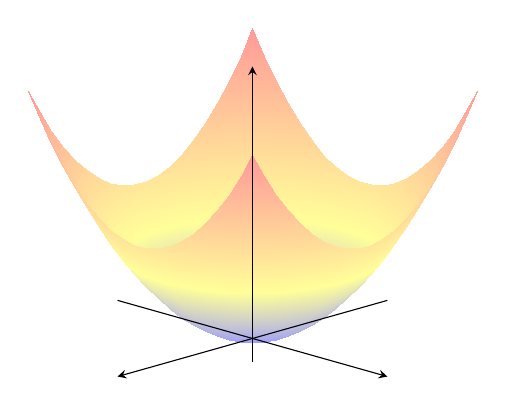
\begin{tikzpicture}
   \begin{axis}[
      view={135}{20},
      axis lines=center,
      enlargelimits,
      axis on top,
      ticks=none,
      samples=20,
      z buffer=sort]
      \addplot3 [
         surf,
         % shader=flat,
         shader=interp,
         fill opacity=.4,
         draw=black
      ] {x*x+y*y};
   \end{axis}
\end{tikzpicture}\\
\textbf{Ellipsoid}\\
$\frac{x^2}{a^2}+\frac{y^2}{b^2}+\frac{z^2}{c^2}=1$\\
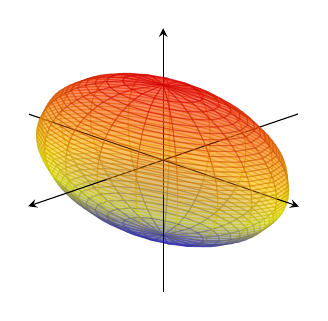
\begin{tikzpicture}
   \begin{axis}
   [view={135}{20},%colormap/blackwhite,
   axis lines=center, axis on top,ticks=none,
   set layers=default,axis equal,
   enlargelimits,
   tick align=inside,
   domain=0:2.00,
   samples=20, 
   z buffer=sort,
   ]
   \addplot3 [surf,opacity=0.4,domain=-1:0,
   domain y=0:360] ({sin(y)*sqrt(1-x^2)},{2*cos(y)*sqrt(1-x^2)},{x});
   \addplot3 [surf,opacity=0.4,domain=0:1,
   domain y=0:360,on layer=axis foreground] ({sin(y)*sqrt(1-x^2)},{2*cos(y)*sqrt(1-x^2)},{x});
   \end{axis}
\end{tikzpicture}
\section{Double Pain D:}
\textbf{Double Riemann Sum}\\
$\lim_{m,n\to\infty}\sum_{i=1}^{m}\sum_{j=1}^{n}f(x_{ij}^*,y_{ij}^*)\triangle A$\\
\textbf{Volume of Solid above Rectangle below z=f(x,y)}\\
$V=\int\int_{R}f(x,y)dA$\\
\textbf{Split Double Integral: Special Case}\\
$f(x,y)=g(x)h(y),\ R=[a,b]\times[c,d]\\V=\int\int_{R}f(x,y)dA\Rightarrow\int_{a }^{b }g(x)dx\int_{c }^{d }h(y)dy$\\
\textbf{Double Integral: Region Type}
\begin{Figure}
   \begin{minipage}{.4\linewidth}
      \centering
      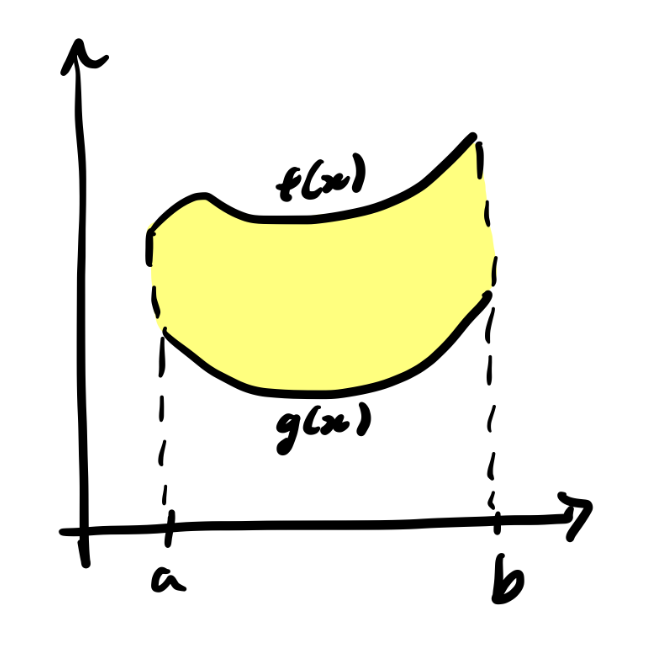
\includegraphics[width=\linewidth]{doubleType1.png}
      \captionsetup{labelformat=empty}
      \captionof{figure}{Type I}
   \end{minipage}
   \begin{minipage}{.4\linewidth}
      \centering
      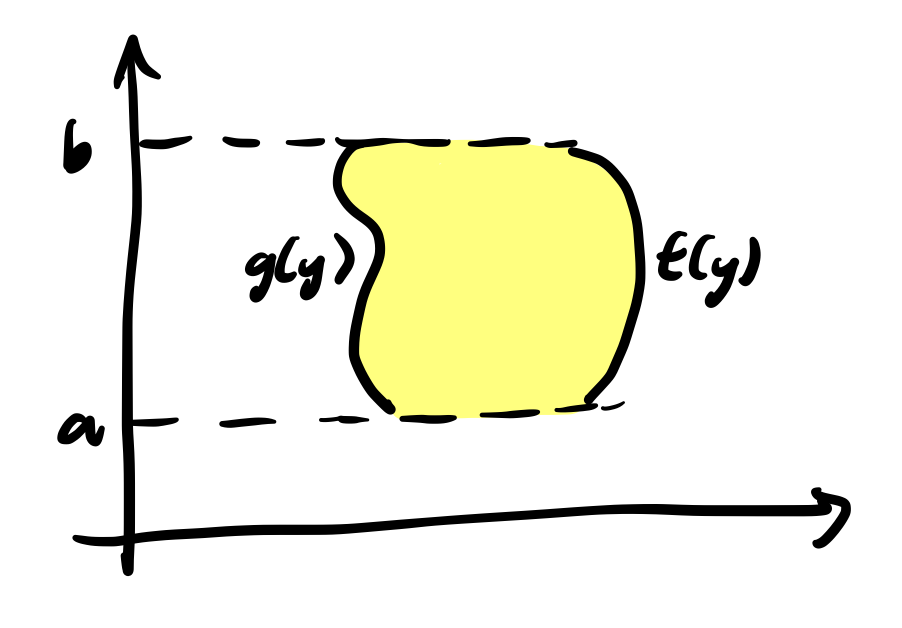
\includegraphics[width=\linewidth]{doubleType2.png}
      \captionsetup{labelformat=empty}
      \captionof{figure}{Type II}
   \end{minipage}
\end{Figure}
Type I: $\int_a^b\int_{g(x)}^{f(x)}f(x,y)dydx$\\
Type II: $\int_a^b\int_{f(y)}^{g(y)}f(x,y)dxdy$\\
\textbf{Decomposition of Domains}\\
$\int\int_Df(x,y)dA=\int\int_{D_1}f(x,y)dA+...+\int\int_{D_n}f(x,y)dA$\\
\textbf{Area/Volume by Iterated Integrals}\\
$A(D)=\int\int_D1dA$\\
$V(S)=\int\int\int_S1dV$\\
\textbf{Rectangle$\mapsto$Polar Coordinates}\\
$r^2=x^+y^2\Rightarrow x=r\cos\theta,y=r\sin\theta$\\
If $f$ is continuous on a polar rectangle\\$R=\{(r,\theta):0\le a\le r\le b,\alpha\le\theta\le\beta\}\wedge0\le\beta-\alpha\le2\pi$\\
$\int\int_Rf(x,y)dA=\int_{\alpha}^{\beta}\int_{a }^{b }f(r\cos\theta,r\sin\theta)rdrd\theta$\\%ANNOTATE HERE REMEMBER THE RRRRRR
\textbf{Surface Area of z=f(x,y)}\\
$\int\int_DdS=\int\int_D\sqrt{f_x^2+f_y^2+1}dA$
\section{Ordinary Differential Equations}
Reading Comprehension\\
\textbf{Separable First Order ODE}\\
$\frac{dy}{dx}=f(x)g(y)$\\
$\int\frac{1}{g(y)}dy=\int f(x)dx+C$\\
\textbf{Non-Separable First Order ODE}\\
Type 1:\\
$\frac{dy}{dx}=g(\frac{y }{x })$\\
Let $v=\frac{y}{x}$. Then $y'=v+xv'$.\\
$v'=\frac{g(v)-v}{x}$
Type 2:\\
$\frac{dy}{dx}=f(ax+by)$\\
Let $u=ax+by$. Then $u'=a+by'$, $y'=\frac{u'-a }{b}$.\\
$\frac{u'-a }{b }=f(u)\Rightarrow u'=bf(u)+a$\\
\textbf{Linear First Order ODE}\\
$\frac{dy}{dx}+P(x)y=Q(x)$\\
Let $I(x)=e^{\int P(x)dx}$.\\
$y\cdot I(x)=\int Q(x)\cdot I(x)dx$\\
\textbf{Bernoulli Equations}\\
$\frac{dy}{dx}+p(x)y=q(x)y^n, n\in\mathbb{R}\backslash\{0,1\}$\\
Let $u=y^{1-n}$. $u'=(1-n)y^{-n}y'$.\\
Multiply both sides by $(1-n)y^{-n}$.\\
$(1-n)y^{-n}y'+(1-n)y^{-n}yp(x)=(1-n)y^{-n}y^nq(x)$\\
$u'+(1-n)p(x)u=(1-n)q(x)$

\end{multicols*}
\end{document}